\documentclass[11pt, twoside, a4paper]{article}
\usepackage{epigraph}
\usepackage{graphicx}
\usepackage[swedish]{babel}

\usepackage[margin=3cm]{geometry}
\usepackage{multicol, float, blindtext, kantlipsum}

\usepackage[citestyle=verbose-ibid, bibstyle=authoryear, natbib=true, url=false, doi=false, isbn=false, backend=biber, labeldateparts]{biblatex}
\AtEveryBibitem{%
  \clearlist{language}%
}
%\usepackage{hyperref}
\addbibresource{bibtex/kandidatarbete.bib}

\usepackage{csquotes}

\usepackage{sectsty}
\subsubsectionfont{\normalfont\itshape}
%\subsectionfont{\normalfont\centering}

\usepackage{titlesec}
\titleformat{\section}
  {\normalfont\LARGE\bfseries}{\thesection}{1em}{}[{}]
  % \titlerule[0.8pt]

\title{Värden och värden:\\
	\large en studie av kollektiv sonifiering
}
\author{Karl Johannes Jondell}
\date{\today}

\begin{document}

% \maketitle

% \begin{abstract}
% Vad handlar detta projekt om?
% \end{abstract}

% \begin{keyword}
% sonifiering \sep% 
% diabetes \sep%
% interaktion
% \end{keyword}

\tableofcontents
\clearpage

\newpage
\begin{multicols}{2}

\section*{Introduktion}
\addcontentsline{toc}{section}{Introduktion}
%\kant[1]

Idéen om att göra musik av mina blodsockervärden föddes samma dag som jag fick en \emph{Freestyle Libre}-mätare (i oktober 2017) vilket är en så kallad kontinuerlig blodsockermätare (en. \emph{continous glucose monitoring}, eller \emph{CGM}). Denna typ av blodsockermätare skiljer sig från tradionella mätare --- som man är tvungen att sticka sig i fingret och på så sätt mäta blodsockret med --- i att den regelbundet gör mätningar, och på så sätt ger en kontinuerlig kurva över ens blodsockervärden. Kurvorna påminde mig om ...

Interaktivitet (\emph{Calling out of context})...

Radio (\emph{Tuning a radio}, etc...)

\subsection*{Bakgrund}
\addcontentsline{toc}{subsection}{Bakgrund}
%Projekt från ettan, diabetes-synth, radiostation, etc.
%\kant[2-2]
\emph{r a d i o q u a l i a}...

\textbf{Sonifiering}, \textbf{autoimmun sjukdom (Diabetes)}, \textbf{interaktivitet}, och \textbf{radio}.


\subsection*{Sonifiering}
\addcontentsline{toc}{subsection}{Sonifiering}
%\kant[3-3]
Sonifiering (eller är det verkligen sonifiering). \footcite[2]{bijsterveld_sonic_2019}
Smalley och spektromorfologin. \footnote{Olika ordningar av \emph{surrogacy},  gestaltandet av \emph{datan}.} Bearbetad data och orginaldata. Sensorfel.

\emph{Audification} \footcite[302]{noauthor_sonification_2011} är en form av sonifiering där mätdatan översätts direkt till ljudkurvor... fyra grupper av data (\emph{sound recording}, \emph{general acoustic}, \emph{physical}, och \textbf{\emph{abstract}})...

\subsubsection*{Det mätbara och det omätbara}
\addcontentsline{toc}{subsubsection}{\textit{Det mätbara och det omätbara}}
Bornemark \footcite{bornemark_det_2018}
Bijsterveld \footcite[100-102]{bijsterveld_sonic_2019}
McLuhan \footcite[2]{mcluhan_understanding_2015}

\subsection*{Diabetes}
\addcontentsline{toc}{subsection}{Diabetes}
%\kant[4-4]

%\subsubsection*{Communities}
%\addcontentsline{toc}{subsubsection}{\textit{Communities}}

\subsubsection*{Blodsockervärden}
\addcontentsline{toc}{subsubsection}{\textit{Blodsockervärden}}
Blodsocker mäts i mmol/L och varierar hos en icke-diabetiker mellan 4 och 6 mmol/L [källa]. Hos en diabetiker kan detta värde variera från under 1 till över 30 mmol/L, och Freestyle Libre-sensorn har ett spann på att mäta från lägst 2,2 till 27,7 mmol/L (annars visar den \emph{LO} respektive \emph{HI}). Freestyle Libre-sensorn mäter kontinuerligt var 15:e minut.

Att s.k. \emph{mappa} denna data till musikaliska parametrar är förstås godtyckligt --- värdena i sig har ingen musikalisk mening --- och bör så vara: det är helt enkelt min konstnärliga gärning som bestämmer hur de förhåller sig till varandra. Även en bearbetad signal går att använda för att styra musiken: interpolation (mellan de diskreta mätpunkterna), variation (FFT, derivator, etc.), stokastiska egenskaper (auto-korrelation etc), statistiska egenskaper (median, medel, etc.). ''\emph{Tid i målområdet}'' och liknande värden kan också vara intressanta att använda, och har medicinsk betydelse.

Det som är viktigt i denna \emph{mappning} är dock att den gestaltade datan --- dvs. musiken --- \textbf{inte} får avslöja något om den underliggande eller bakomliggande (mät)datan. Dels är det en integritetsfråga, som diskuteras vidare nedan, dels är det en förutsättning för detta projekt: det existerar inga \emph{bra} eller \emph{dåliga} värden. Själva delningen av värdena är det viktiga.

\subsubsection{Förhållandet till mätandet}
I sin text \emph{Det autoimmuna jaget --- om att sätta gränser} \footcite[286]{arvidson_det_2016} skriver Mats Arvidson om kravet som diabetiker på disciplin \emph{och} prestation.

\section*{Process}
\addcontentsline{toc}{subsection}{Process}
Beskrivning/dokumentation av tekniken...

% \begin{figure}[H]
% \centering
% 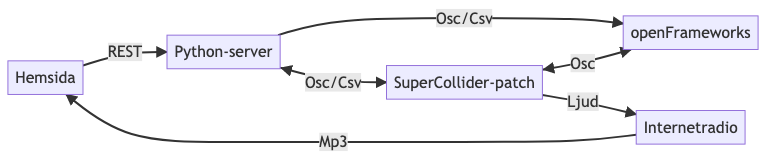
\includegraphics[width=0.5\textwidth]{../media/flowchart.png}
% \caption{Översiktsdiagram av system}
% \end{figure}

\subsection*{SuperCollider-system}
\addcontentsline{toc}{subsection}{SuperCollider-system}
Varje instans av mätdata existerar som ett \emph{objekt} (motsvarande en ljudkälla, inte schaefferiansk) i musiken, objekten har vissa attribut (såsom register, spatiell kodning, etc). Även kodat binauralt (via \emph{Ambisonics}). Klassen har en Osc-tolkarfunktion (\textbf{eller} CSV-filläsare, om asynkron).

\section*{Musiken}
\addcontentsline{toc}{section}{Musiken}
Den konstnärliga friheten. Hur pass mycket kontroll som överlåtes till \enquote{serien} (i detta fall blodsockervärdet). Behöver musiken gestalta, spegla, estetisera erfarenheten som diabetiker? Eller vara intresseväckande, tillgänglig, \enquote{relaterbar}? 

\subsection*{Rumslighet}
\addcontentsline{toc}{subsection}{Rumslighet}
En \enquote{kör} av blodsockervärden, spatialiserade i nån mening för att ge en känsla av påverkan eller åverkan på musiken. 

Konsertupplevelse (i Lilla salen? spela ett utdrag ur liveströmmen...)

\subsection*{Temporalitet}
\addcontentsline{toc}{subsection}{Temporalitet}
Den tidsmässiga uppfattningen av musiken. En 24/7 livestream av musiken (hur utgörs lyssnadet? formen? \emph{Slow as possible}, \emph{Longplayer} och liknande...)

\subsection*{Generativt}
\addcontentsline{toc}{subsection}{Generativt}
Musiken är generativ. Serialism?

\section*{Sammanfattning}
\addcontentsline{toc}{section}{Sammanfattning}
Lärdomar etc...

\end{multicols}

\twocolumn

\printbibliography[type=book,title={Böcker}]
\printbibliography[type=article,title={Artiklar}]

\end{document}

